\begin{document}
\maketitle

\begin{frame}
  \titlepage
\end{frame}

\cleardoublepage

\tableofcontents

\cleardoublepage

\section{Introduction}

\note{As you can imagine, the truth is in between these extremes}

\note{
  A few words about myself:
}

\begin{frame}{Me}
\begin{itemize}
\item Nick name: racke
\item Self employed programmer since 1998
\item Web applications
\item Ecommerce
\item Database
\item Customers in Germany, Switzerland, USA, ...
\end{itemize}
\end{frame}

\note{
  One of my customers is the US Department of State.
  I'm responsible for a number of their web sites, for example
  the procurement solution eShop.
}

\begin{frame}{eShop}
\begin{figure}[!ht]
\centering
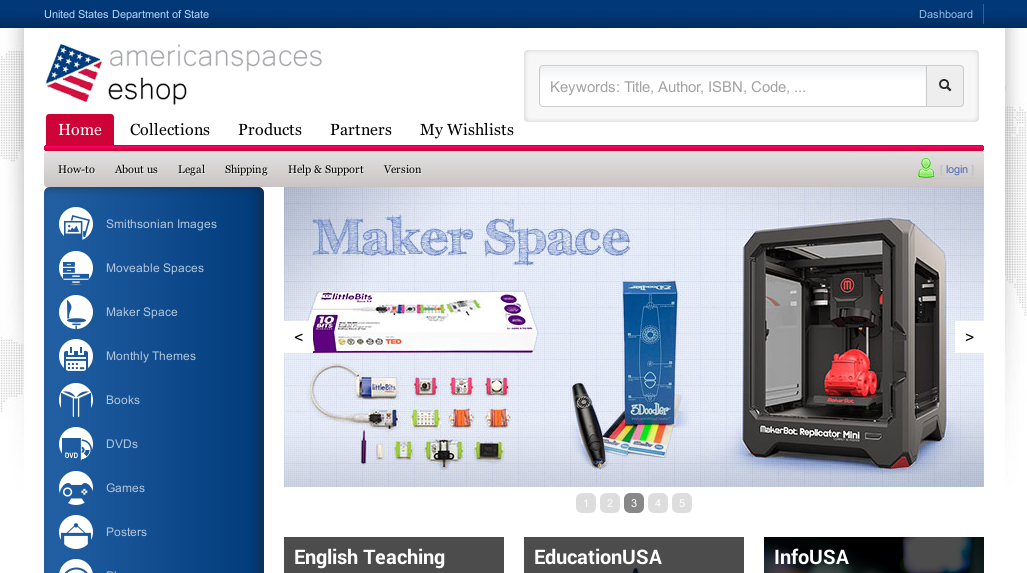
\includegraphics[width=1\linewidth]{img/eshop.png}
\end{figure}
\end{frame}

\begin{frame}{Interchange}
\begin{figure}[!ht]
\centering

\includegraphics[width=1\linewidth]{img/interchange.jpg}
\end{figure}
\end{frame}

\begin{frame}{Interchange}
\begin{itemize}
\item Embedded SQL
\item \sout{Modern Perl}
\end{itemize}
\end{frame}

\begin{frame}{Dancer / DBIx::Class}
\begin{itemize}
\item Dancer
\item DBIx::Class
\item Interchange6
\end{itemize}
\end{frame}

\note{We organized the second Perl Dancer conference October,}

\begin{frame}{Perl Dancer Conference}
\begin{figure}[!ht]
\centering

\includegraphics[width=1\linewidth]{img/perl-dancer-homepage-logo.png}
\end{figure}
\end{frame}

\note{where he had also a one day DBIx::Class training.

Here you see my co-trainers, ribasushi (mastermind behind
DBIx::Class) and Peter Mottram doing the last preparations
for the training:
}

\begin{frame}{DBIx::Class Training}
\begin{figure}[!ht]
\centering
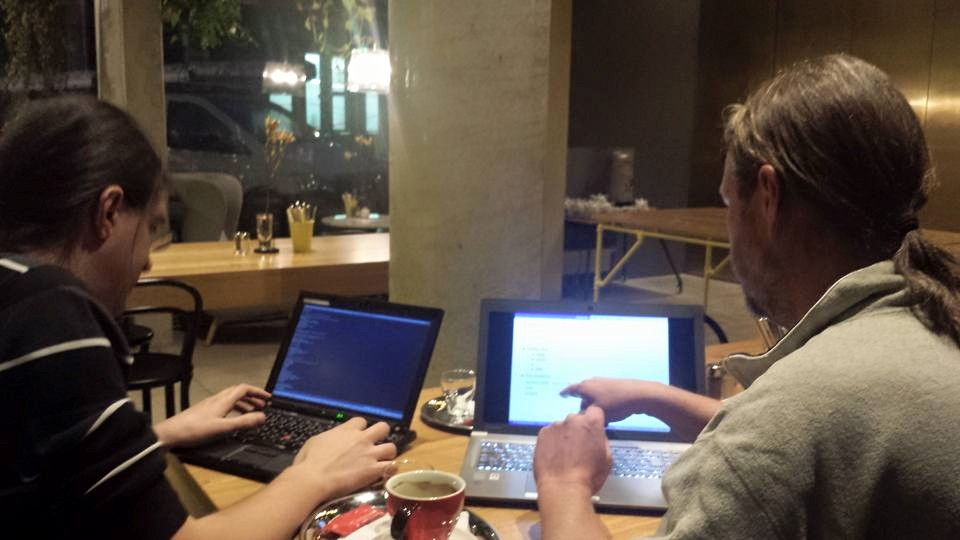
\includegraphics[width=1\linewidth]{img/training-preps.jpg}
\end{figure}
\end{frame}

\note{Baltimore Outage April}

\begin{frame}[fragile]{Conference website}
\begin{itemize}
\item ACT 2014
\begin{itemize}
\item Legacy code
\item No server control
\end{itemize}
\item www.perl.dance 2015
\begin{itemize}
\item Dancer / DBIx::Class
\item Most ACT features + new features
\item \url{https://github.com/interchange/Perl-Dancer-Conference}
\end{itemize}
\end{itemize}
\end{frame}

\begin{frame}{DBIx::Class Features}
\begin{itemize}
\item OO instead of SQL
\item Abstracts different SQL implementations
\item Business Logic
\item Performance
\item ``ResultSet'' features
\item Ecosystem
\begin{itemize}
\item IRC / Mailing list
\item Components
\item Helpers
\end{itemize}
\end{itemize}
\end{frame}

\subsection{Business Logic}
\begin{frame}{Business Logic}
% move business logic into schema
% https://pixabay.com/en/gear-gears-euro-forex-dollar-384743/
\begin{figure}[!ht]
\centering

\includegraphics[width=0.75\linewidth]{img/business-logic.jpg}
\end{figure}
\end{frame}

\begin{frame}{Business Logic Benefits}
\begin{itemize}
\item Multiple Consumers
\begin{itemize}
\item Web application(s)
\item Cron jobs, scripts
\item Test environments
\end{itemize}
\item Hide Implementation
\begin{itemize}
\item SQL Dialects
\item Application View
\end{itemize}
\item Changes / DRY
\end{itemize}
\end{frame}

\subsection{Performance}

All the experience, tests and different areas in which 
DBIx::Class is applied makes it perform better than
handwritten SQL is most cases.

\begin{frame}{Performance}
\begin{itemize}
\item Experience
\item Test results
\item Use cases
\end{itemize}
\end{frame}

\begin{frame}[fragile]{Literal SQL}
\begin{lstlisting}
$schema->resultset('PlaceVisited')->search(
{
  users_id => {
    -in => \[
       'SELECT users_id FROM users WHERE users_id > ?',
       2
    ]
  }
});
\end{lstlisting}
\end{frame}

But please don't complain if that leads to headache
and wasted time better spent on proper DBIx::Class
code.

\begin{frame}{SQL Headache}
% https://pixabay.com/en/stress-man-hand-flame-burn-fire-864141/
\begin{figure}[!ht]
\centering
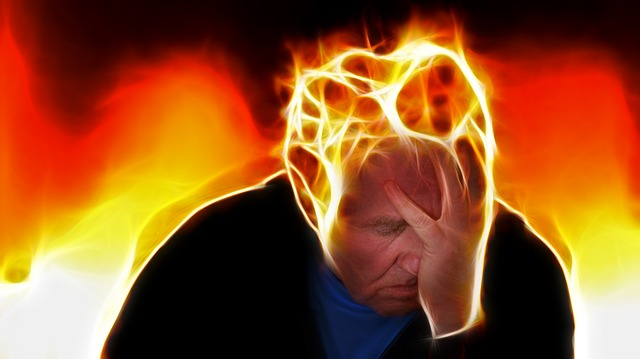
\includegraphics[width=1\linewidth]{img/stress.jpg}
\end{figure}
\end{frame}

\section{Set Based DBIx::Class}

\note{The most important feature of DBIx::Class is the Resultset,
which we will examine through an example soon.}

\begin{frame}[fragile]{Set Based DBIx::Class}
\begin{figure}[!ht]
\centering
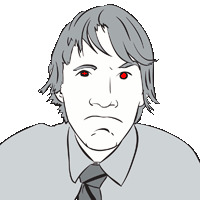
\includegraphics[width=0.4\linewidth]{img/frew.png}
\caption{Arthur Axel "fREW" Schmidt}
\end{figure}
\centering
\href{http://www.perladvent.org/2012/2012-12-21.html}{http://www.perladvent.org/2012/2012-12-21.html}
\end{frame}

\begin{frame}{Set Based DBIx::Class}
\begin{itemize}
\item ORM
\begin{itemize}
\item Objects
\item Abstracts SQL
\item ...
\end{itemize}
\item ResultSet
\begin{itemize}
\item Chaining
\item Relationship Traversal
\item Correlated Subqueries
\item ...
\end{itemize}
\end{itemize}
\end{frame}

\begin{frame}{Using ResultSet}
\begin{itemize}
\item Simple SQL query
\item Turn into DBIx::Class search
\item Use ResultSet features
\end{itemize}
\end{frame}

\begin{frame}[fragile]{Simple SQL query}
List of talks on last day of Perl Dancer Conference:
\begin{lstlisting}
SELECT talks_id, author_id, conferences_id, duration,
title, tags, abstract, url, comments, accepted, confirmed, 
lightning, scheduled, start_time, room, survey_id 
FROM talks 
WHERE accepted is TRUE 
AND conferences_id = 1 
AND room != '' 
AND start_time >= '2015-10-22 00:00:00'
AND start_time <= '2015-10-23 00:00:00'
\end{lstlisting}
\end{frame}

\begin{frame}[fragile]{Simple SQL query}
With DBIx::Class:
\begin{lstlisting}
my $talks = $schema->resultset('Talk')->search(
    {
        -bool          => 'accepted',
        conferences_id => 1,
        room           => { '!=' => '' },
        start_time     => {
            '>=' => '2015-10-22 00:00:00'
            '<=' => '2015-10-23 00:00:00'
            },
    },
);
\end{lstlisting}
\end{frame}


\begin{frame}[fragile]{Truth of ResultSet}
% \centering
\sout{ResultSet}

\begin{lstlisting}
isa(Query Plan);
\end{lstlisting}

\end{frame}

\begin{frame}[fragile]{Truth of ResultSet}

This doesn't execute SQL:

\begin{lstlisting}
my $talks = $schema->resultset('Talk')->search(...);
\end{lstlisting}

This does:

\begin{lstlisting}
my $first_talk = $schema->resultset('Talk')
                 ->search(...)->first;
\end{lstlisting}

\end{frame}

\section{Composability}

Composability means that you don't need to construct the
complete at once, but compose it together, e.g with
chaining.

The underlying mechanism is that \verb|->search| on a
ResultSet actually doesn't search.

\subsection{Tickets}

\begin{frame}{Tickets}
\begin{figure}[!ht]
\centering
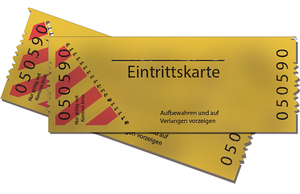
\includegraphics[width=0.8\linewidth]{img/cinema-ticket.png}
\end{figure}
\end{frame}

\begin{frame}{Tickets}
\begin{figure}[!ht]
\centering
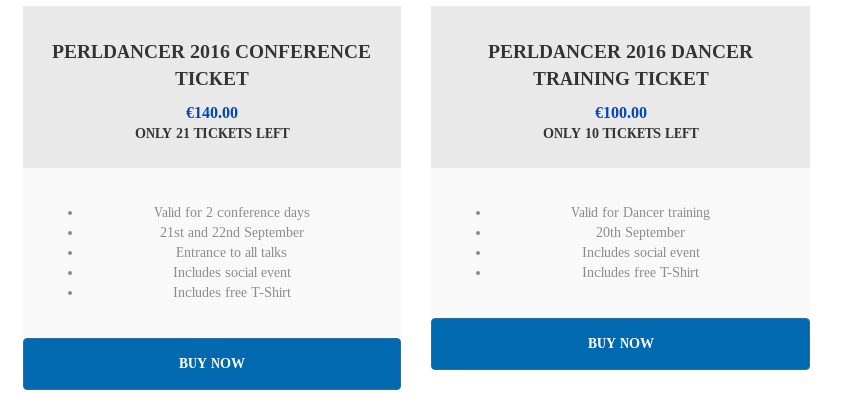
\includegraphics[width=0.8\linewidth]{img/ticket-view.png}
\end{figure}
\end{frame}

\begin{frame}[fragile]{Tickets with inventory}
\begin{itemize}
\item Conference
\item Tickets
\item Conference Tickets
\item Inventory
\end{itemize}
\end{frame}

\begin{frame}[fragile]{Tickets with inventory}
\begin{lstlisting}

SELECT ticket.sku, ticket.name, 
  ticket.short_description, ticket.description, 
  ticket.price, inventory.sku, inventory.quantity 
  FROM conference_tickets me 
  JOIN products ticket 
    ON ticket.sku = me.sku 
  LEFT JOIN inventories inventory 
    ON inventory.sku = ticket.sku 
WHERE me.conferences_id = '2' AND ticket.active = '1'

\end{lstlisting}
\end{frame}

\begin{frame}{Chaining}
  \begin{figure}[!ht]
    \begin{center}
      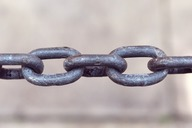
\includegraphics{img/chains.jpg}
    \end{center}
  \end{figure}
\end{frame}

\begin{frame}[fragile]{Tickets}

\begin{lstlisting}
  $tickets = $schema->resultset( 'Conference' )
     ->find( {name => 'Perl Dancer Conference 2016'}, )
     ->tickets
     ->active
     ->prefetch('inventory');
\end{lstlisting}
\end{frame}

\begin{frame}[fragile]{Tickets - Relationship Traversal}
\begin{lstlisting}
package PerlDance::Schema::Result::Conference;

...

has_many
  conference_tickets =>
     'PerlDance::Schema::Result::ConferenceTicket',
  "conferences_id";

many_to_many tickets => "conference_tickets", "ticket";

\end{lstlisting}
\end{frame}

\begin{frame}[fragile]{Tickets - Predefined Search}
\begin{lstlisting}

package Interchange6::Schema::ResultSet::Product;

...

sub active {
    return $_[0]->search({ $_[0]->me('active') => 1 });
}

\end{lstlisting}
\end{frame}

\begin{frame}[fragile]{Tickets - Helpers}

DBIx::Class::Helper::ResultSet::Shortcut

\begin{lstlisting}
$tickets_rs->search( undef, { prefetch => 'inventory' } );

$tickets_rs->prefetch('inventory');
\end{lstlisting}
\end{frame}

\subsection{Talks with number of attendees}

\begin{frame}{Talks with number of attendees}
\begin{figure}[!ht]
\centering
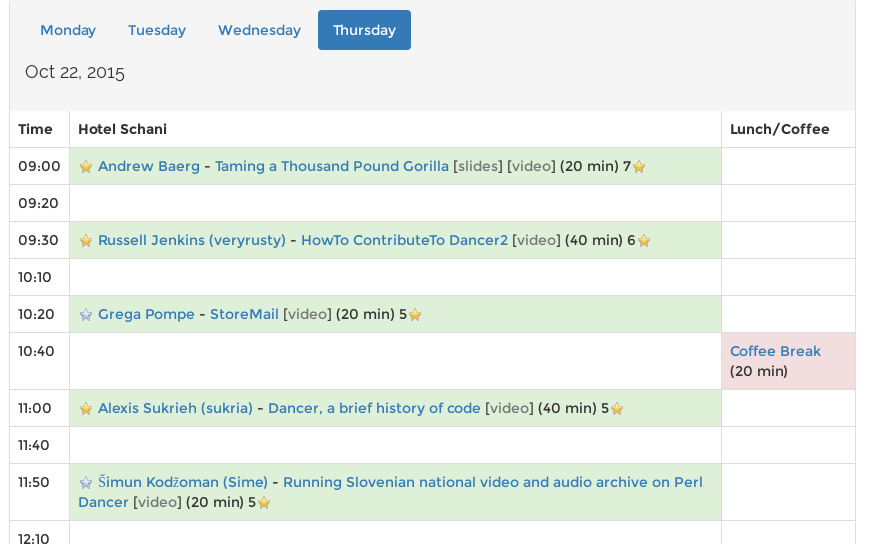
\includegraphics[width=0.8\linewidth]{img/schedule2015.png}
\end{figure}
\end{frame}

\begin{frame}[fragile]{The naive way}
\begin{lstlisting}
my @data = map +{
   %{ $_->as_hash },
   attendee_count => $_->attendee_talks->count,
}, $talks_rs->all
\end{lstlisting}

Problem: one extra query per talk

Other solution: \verb|GROUP BY| \textit{(not recommended)}
\end{frame}

\begin{frame}[fragile]{Correlated Subqueries}
\begin{lstlisting}
package PerlDance::Schema::ResultSet::Talk;

sub with_attendee_count {
  my $self = shift;

  $self->search(
    undef,
      {
        '+columns' => {
           attendee_count =>
             $self->correlate('attendee_talks')
               ->count_rs
               ->as_query
        }
      }
  );
}
\end{lstlisting}
\end{frame}

\begin{frame}[fragile]{Correlated Subqueries}
\begin{lstlisting}
( 
  SELECT COUNT( * ) 
  FROM "attendee_talks" "attendee_talks_alias" 
  WHERE "attendee_talks_alias"."talks_id" = "me"."talks_id"
), 
\end{lstlisting}
\end{frame}

\begin{frame}[fragile]{Correlated Subqueries}
\begin{lstlisting}
my $talks = rset('Talk')->search(
  {
    accepted       => 1,
    conferences_id => setting('conferences_id'),
    room           => { '!=' => '' },
    start_time     => {
      '!=' => undef,
      '>=' => $schema->format_datetime($dt_date),
      '<=' =>
         $schema->format_datetime( 
           $dt_date->clone->add( days => 1 ) )
    },
  },
  {
    order_by => 'start_time',
    prefetch => 'author',
  }
)->with_attendee_count;
\end{lstlisting}
\end{frame}

\begin{frame}[fragile]{Correlated Subqueries}
\begin{lstlisting}
DBIx::Class::Helper::ResultSet::CorrelateRelationship
\end{lstlisting}
\end{frame}

\begin{frame}{Talks with number of attendees}
\begin{figure}[!ht]
\centering
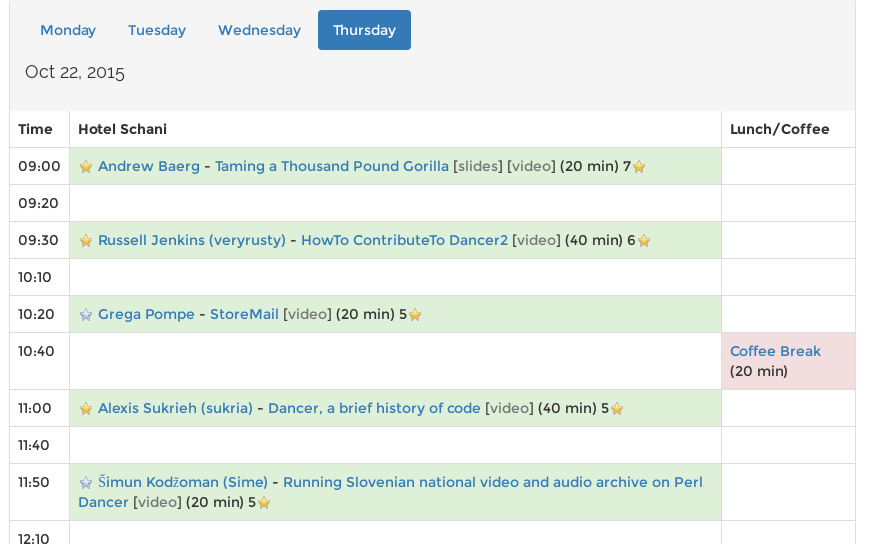
\includegraphics[width=0.8\linewidth]{img/schedule2015.png}
\end{figure}
\end{frame}

\begin{frame}[fragile]{Correlated Subqueries}
\begin{lstlisting}
sub with_attendee_status {
  my ( $self, $users_id ) = @_;

  $self->search(
    undef,
    {
      '+columns' => {
        attendee_status => 
          $self->correlate('attendee_talks')->search(
          {
            users_id => $users_id
          }
        )->count_rs->as_query
      }
    }
  );
}
\end{lstlisting}
\end{frame}

\begin{frame}[fragile]{Correlated Subqueries}
\begin{lstlisting}
$talks = $talks->with_attendee_status( $user->id );
\end{lstlisting}

\begin{lstlisting}
( 
  SELECT COUNT( * )
    FROM attendee_talks attendee_talks_alias
    WHERE attendee_talks_alias.talks_id = me.talks_id
    AND users_id = '4'
),
\end{lstlisting}
\end{frame}

\begin{frame}[fragile]{Correlated Subqueries}
\begin{lstlisting}
      
$talks = $talks->with_attendee_status( $user->id );

\end{lstlisting}
\end{frame}

\begin{frame}[fragile]{Correlated Subqueries}
\begin{lstlisting}
my $talks = rset('Talk')->search(
  {
    accepted       => 1,
    conferences_id => setting('conferences_id'),
    room           => { '!=' => '' },
    start_time     => {
      '!=' => undef,
      '>=' => $schema->format_datetime($dt_date),
      '<=' =>
         $schema->format_datetime( 
           $dt_date->clone->add( days => 1 ) )
    },
  },
  {
    order_by => 'start_time',
    prefetch => 'author',
  }
)->with_attendee_count->with_attendee_status( $user->id );
\end{lstlisting}
\end{frame}

\begin{frame}[fragile]{Correlated Subqueries}
\begin{lstlisting}
SELECT me."talks_id", me."author_id", me."conferences_id", me."duration", me."title", me."tags", me."abstract", me."url", me."video_url", me."comments", me."organiser_notes", me."accepted", me."confirmed", me."lightning", me."scheduled", me."start_time", me."room", me."created", me."last_modified", me."survey_id", ( 
    SELECT COUNT( * ) 
      FROM "attendee_talks" "attendee_talks_alias" 
    WHERE "attendee_talks_alias"."talks_id" = me."talks_id"
   ), ( 
    SELECT COUNT( * ) 
      FROM "attendee_talks" "attendee_talks_alias" 
    WHERE "attendee_talks_alias"."talks_id" = me."talks_id" AND "users_id" = '4'
   ), "author"."users_id", "author"."username", "author"."nickname", "author"."email", "author"."password", "author"."first_name", "author"."last_name", "author"."last_login", "author"."fail_count", "author"."reset_expires", "author"."reset_token", "author"."is_anonymous", "author"."created", "author"."last_modified", "author"."active", "author"."bio", "author"."media_id", "author"."monger_groups", "author"."pause_id", "author"."guru_level", "author"."t_shirt_size" 
  FROM "talks" me LEFT JOIN "users" "author" 
    ON "author"."users_id" = me."author_id" 
WHERE "accepted" = '1' AND "conferences_id" = '1' AND "room" != '' 
AND "start_time" IS NOT NULL AND "start_time" <= '2015-10-23 00:00:00' 
AND "start_time" >= '2015-10-22 00:00:00' 
ORDER BY "start_time"
\end{lstlisting}
\end{frame}

\begin{frame}[fragile]{Predefined Searches}
\begin{lstlisting}
my $talks = rset('Talk')->search(
  {
    accepted       => 1,
    conferences_id => setting('conferences_id'),
    room           => { '!=' => '' },
    start_time     => {
      '!=' => undef,
      '>=' => $schema->format_datetime($dt_date),
      '<=' =>
         $schema->format_datetime( 
           $dt_date->clone->add( days => 1 ) )
    },
  },
  {
    order_by => 'start_time',
    prefetch => 'author',
  }
)->with_attendee_count->with_attendee_status( $user->id );
\end{lstlisting}
\end{frame}


\begin{frame}[fragile]{Predefined Searches}
\begin{lstlisting}
package PerlDance::Schema::ResultSet::Talk;

sub scheduled_for {
  my ( $self, $dt_date ) = @_;
  my $schema = $self->result_source->schema;

  $self->search(
    {
      start_time     => {
        '!=' => undef,
        '>=' => $schema->format_datetime( $dt_date ),
        '<=' =>
                $schema->format_datetime( 
                  $dt_date->clone->add( days => 1 ) ),
      },
    }
  );
}
\end{lstlisting}
\end{frame}

\begin{frame}[fragile]{Predefined Searches}
\begin{lstlisting}
my $talks = rset('Talk')->search(
  {
    accepted       => 1,
    conferences_id => setting('conferences_id'),
    room           => { '!=' => '' },
  },
  {
    order_by => 'start_time',
    prefetch => 'author',
  }
)
->scheduled_for( $dt_date )
->with_attendee_count
->with_attendee_status( $user->id );
\end{lstlisting}
\end{frame}

\section{Conclusion}

\begin{frame}{Conclusion}
\begin{itemize}
\item Resources
\item Slides
\item Perl Dancer Conference 2016
\item Questions
\end{itemize}
\end{frame}

\subsection{Resources}
\begin{frame}[fragile]{Resources}
\begin{itemize}
\item Extensive Documentation
\begin{itemize}
\item \verb|DBIx::Class::Manual::*|
\item \verb|DBIx::Class::Manual::ResultClass|
\item \verb|DBIx::Class::ResultSet|
\item \verb|DBIx::Class::Relationship::*|
\end{itemize}
\item \href{http://www.perladvent.org/2012/2012-12-21.html}
{Perl Advent Calendar 2012: Set-based DBIx::Class}
by fRew
\end{itemize}
\end{frame}

\subsection{Slides}
\begin{frame}{Slides}
Slides:
\url{https://www.linuxia.de/talks/alpine2016/dbic-pr-en-beamer.pdf}
\end{frame}

\subsection{Perl Dancer Conference 2016}
\begin{frame}{Perl Dancer Conference 2016}
\begin{figure}[!ht]
\centering

\includegraphics[width=1\linewidth]{img/perl-dancer-homepage-logo-2016.png}
\end{figure}
\end{frame}

\begin{frame}{Dancer Training}
\begin{figure}[!ht]
\centering

\includegraphics[width=0.6\linewidth]{img/sawyer.png}
\end{figure}
\end{frame}

\begin{frame}{New People}
\begin{figure}[!ht]
\centering
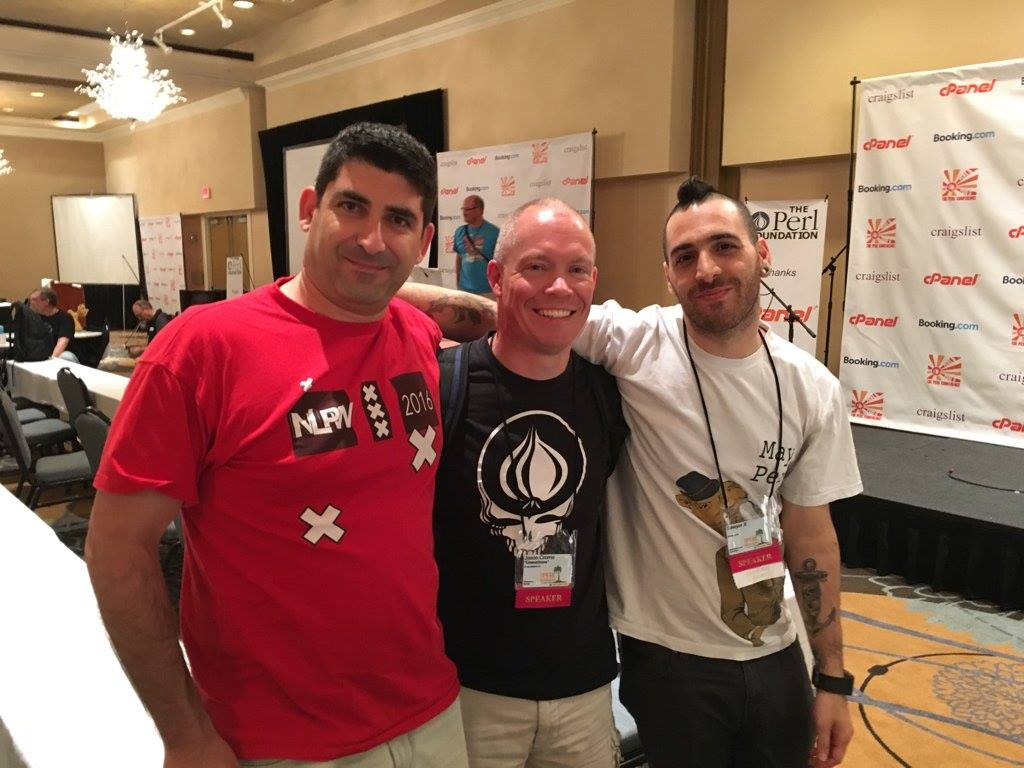
\includegraphics[width=1\linewidth]{img/crowd.png}
\end{figure}
\end{frame}

\subsection{Finish}

\begin{frame}{Questions}
\centering
Questions ?
\end{frame}

\end{document}

%%% Local Variables: 
%%% mode: latex
%%% TeX-master: t
%%% End: 
